\section{适配器与组合}

\subsection{适配器模式}

\subsubsection{模式动机}
在软件开发中采用类似于电源适配器的设计和编码技巧被称为适配器模式。
\begin{itemize}
    \item 通常情况下,客户端可以通过目标类的接口访问它所提供的服务。有时,现有的类可以满足客户类的功能需要,但是它所提供的接口不一定是客户类所期望的,这可能是因为现有类中方法名与目标类中定义的方法名不一致等原因所导致的。
    \item 在这种情况下,现有的接口需要转化为客户类期望的接口,这样保证了对现有类的重用。如果不进行这样的转化,客户类就不能利用现有类所提供的功能,适配器模式可以完成这样的转化。
\end{itemize}

在适配器模式中可以定义一个包装类,包装不兼容接口的对象,这个包装类指的就是\textbf{适配器}(Adapter),它所包装的对象就是\textbf{适配者}(Adaptee),即被适配的类。

适配器提供客户类需要的接口,\textbf{适配器的实现就是把客户类的请求转化为对适配者的相应接口的调用}。也就是说:当客户类调用适配器的方法时,在适配器类的内部将调用适配者类的方法,而这个过程对客户类是透明的,客户类并不直接访问适配者类。因此,\textbf{适配器可以使由于接口不兼容而不能交互的类可以一起工作}。这就是适配器模式的模式动机。

\subsubsection{模式定义}
适配器模式(Adapter Pattern):将一个接口转换成客户希望的另一个接口,适配器模式使接口不兼容的那些类可以一起工作,其别名为包装器(Wrapper)。适配器模式既可以作为类结构型模式,也可以作为对象结构型模式。

\subsubsection{模式结构}
适配器模式包含如下角色:
\vspace{-0.8em}
\begin{multicols}{2}
    \begin{itemize}
        \item Target:目标抽象类
        \item Adapter:适配器类
        \item Adaptee:适配者类
        \item Client:客户类
    \end{itemize}
\end{multicols}
\vspace{-1em}

\begin{figure}[H]
	\centering
    \vspace{-0.5em}
	\subfloat[对象适配器模式结构]{
	\begin{minipage}[t]{0.48\linewidth}
		\centering
		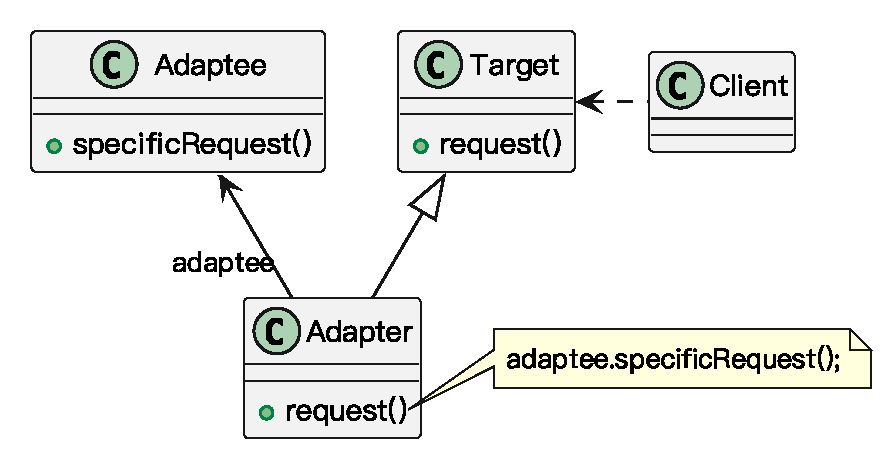
\includegraphics[width=0.97\linewidth]{images/对象适配器模式结构.eps}
	\end{minipage}
	}
    \subfloat[类适配器模式结构]{
    \begin{minipage}[t]{0.48\linewidth}
        \centering
        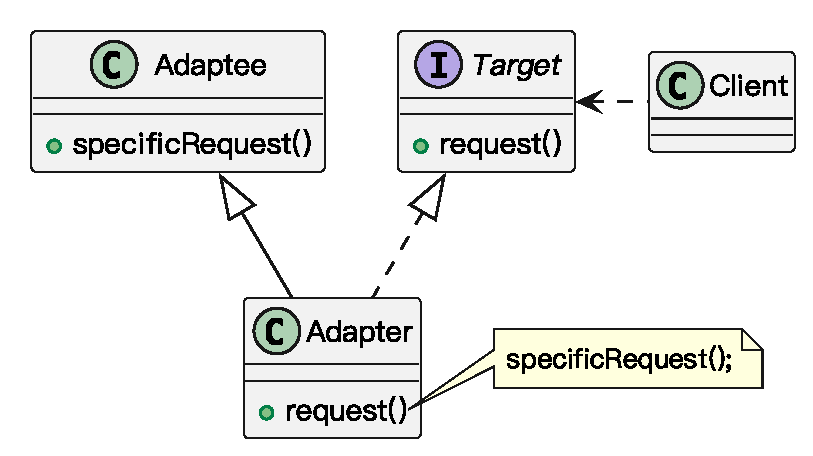
\includegraphics[width=0.97\linewidth]{images/类适配器模式结构.eps}
    \end{minipage}
    }
	\centering
    \vspace{-1em}
\end{figure}

\subsubsection{模式分析}
适配器模式典型代码如下:
\begin{figure}[H]
    \vspace{-0.5em}
	\centering
	\includegraphics[width=0.9\textwidth]{images/适配器模式分析.pdf}
    \vspace{-1em}
\end{figure}

\subsubsection{模式实例}
仿生机器人:现需要设计一个可以模拟各种动物行为的机器人,在机器人中定义了一系列方法,如机器人叫喊方法\sverb|cry()|、机器人移动方法\sverb|move()|\;等。如果希望在不修改已有代码的基础上使得机器人能够像狗一样叫,像狗一样跑,使用适配器模式进行系统设计。
\begin{figure}[H]
    \vspace{-0.5em}
	\centering
	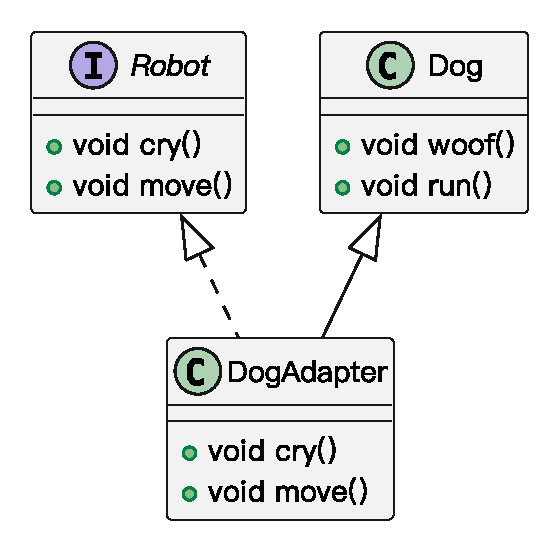
\includegraphics[width=0.3\textwidth]{images/适配器模式实例1.eps}
    \vspace{-1em}
\end{figure}

加密适配器:某系统需要提供一个加密模块,将用户信息(如密码等机密信息)加密之后再存储在数据库中,系统已经定义好了数据库操作类。为了提高开发效率,现需要重用已有的加密算法,这些算法封装在一些由第三方提供的类中,有些甚至没有源代码。使用适配器模式设计该加密模块,实现在不修改现有类的基础上重用第三方加密方法。
\begin{figure}[H]
    \vspace{-0.5em}
	\centering
	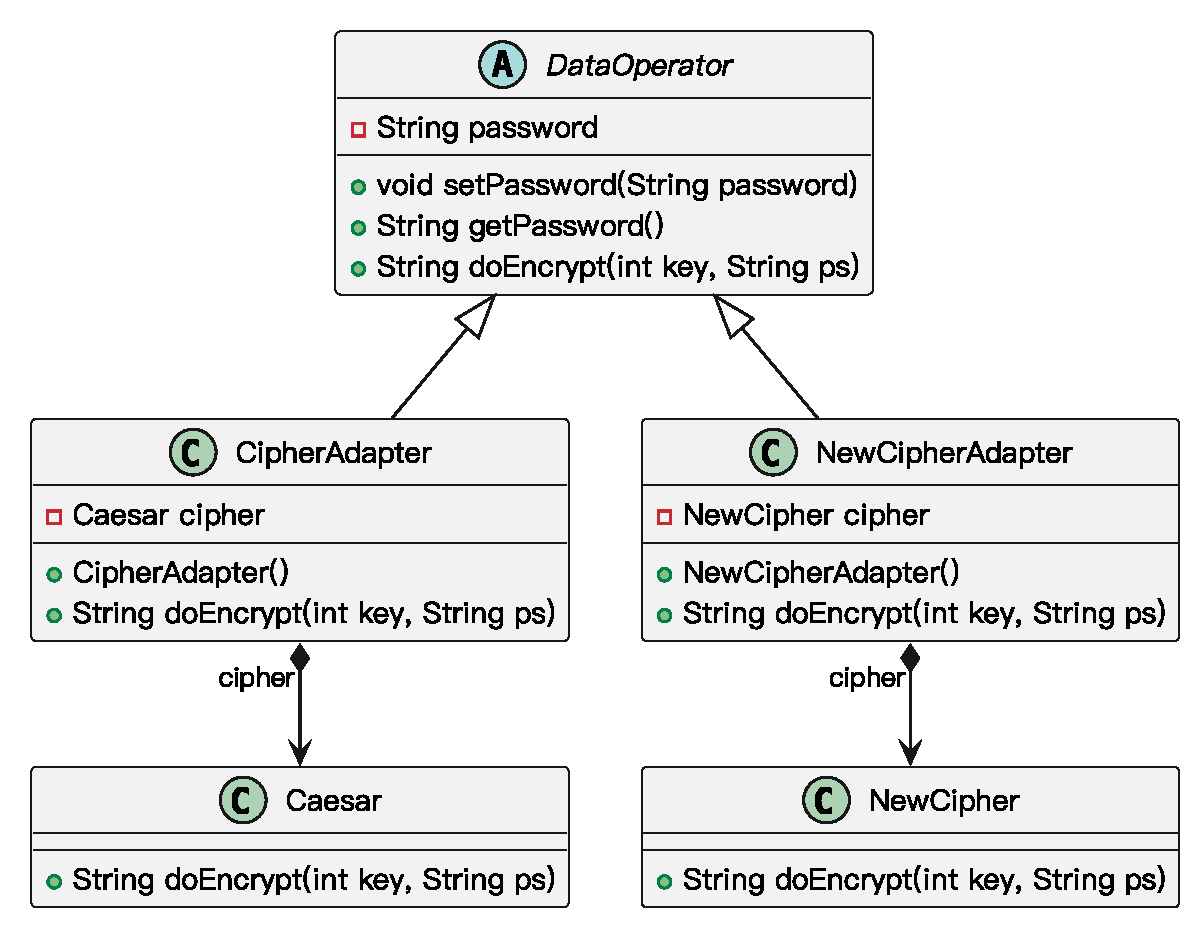
\includegraphics[width=0.75\textwidth]{images/适配器模式实例2.eps}
    \vspace{-1em}
\end{figure}

\subsubsection{模式优缺点}
适配器模式的优点:
\begin{itemize}
    \item \textbf{将目标类和适配者类解耦},通过引入一个适配器类来重用现有的适配者类,而无须修改原有代码。
    \item \textbf{增加了类的透明性和复用性},将具体的实现封装在适配者类中,对于客户端类来说是透明的,而且提高了适配者的复用性。
    \item \textbf{灵活性和扩展性都非常好},通过使用配置文件,可以很方便地更换适配器,也可以在不修改原有代码的基础上增加新的适配器类,完全符合“开闭原则”。
\end{itemize}

类适配器模式还具有如下优点:
\begin{itemize}
    \item 由于适配器类是适配者类的子类,因此\textbf{可以在适配器类中置换一些适配者的方法},使得适配器的灵活性更强。
\end{itemize}

对象适配器模式还具有如下优点:
\begin{itemize}
    \item 一个对象适配器可以把多个不同的适配者适配到同一个目标,也就是说,\textbf{同一个适配器可以把适配者类和它的子类都适配到目标接口}。
\end{itemize}

类适配器模式的缺点如下:
\begin{itemize}
    \item 对于Java、C\#等不支持多重继承的语言,一次最多只能适配一个适配者类,而且目标抽象类只能为抽象类,不能为具体类,\textbf{其使用有一定的局限性},不能将一个适配者类和它的子类都适配到目标接口。
\end{itemize}

对象适配器模式的缺点如下:
\begin{itemize}
    \item 与类适配器模式相比,\textbf{要想置换适配者类的方法就不容易}。如果一定要置换掉适配者类的一个或多个方法,就只好先做一个适配者类的子类,将适配者类的方法置换掉,然后再把适配者类的子类当做真正的适配者进行适配,实现过程较为复杂。
\end{itemize}

\subsubsection{模式适用环境}
在以下情况下可以使用适配器模式:
\begin{itemize}
    \item 系统需要使用现有的类,而这些类的接口不符合系统的需要。
    \item 想要建立一个可以重复使用的类,用于与一些彼此之间没有太大关联的一些类,包括一些可能在将来引进的类一起工作。
\end{itemize}

\subsubsection{模式应用}
\ding{172} Sun公司在1996年公开了Java语言的数据库连接工具JDBC,JDBC使得Java语言程序能够与数据库连接,并使用SQL语言来查询和操作数据。JDBC给出一个客户端通用的抽象接口,每一个具体数据库引擎(如SQL Server、Oracle、MySQL等)的JDBC驱动软件都是一个介于JDBC接口和数据库引擎接口之间的适配器软件。抽象的JDBC接口和各个数据库引擎API之间都需要相应的适配器软件,这就是为各个不同数据库引擎准备的驱动程序。

\ding{173} 在JDK类库中也定义了一系列适配器类,如在\sverb|com.sun.imageio.plugins.common|\; 包中定义的\sverb|Input| \verb|StreamAdapter|\;类,用于包装\sverb|ImageInputStream|\;接口及其子类对象。
\begin{lstlisting}
public class InputStreamAdapter extends InputStream{
    ImageInputStream stream;
    public InputStreamAdapter(ImageInputStream stream) {
        super();
        this.stream = stream;
    }
    public int read() throws IOException {
        return stream.read();
    }
    public int read(byte b[], int off, int len) throws IOException {
        return stream.read(b, off, len);
    }
}
\end{lstlisting}

\subsubsection{模式扩展}

\paragraph*{默认适配器模式(缺省适配器模式)}~{} \par
当不需要全部实现接口提供的方法时,可先设计一个抽象类实现接口,并为该接口中每个方法提供一个默认实现(空方法),那么该抽象类的子类可有选择地覆盖父类的某些方法来实现需求,它适用于一个接口不想使用其所有的方法的情况。因此也称为单接口适配器模式。
\begin{figure}[H]
	\centering
    \vspace{-0.5em}
	\subfloat{
	\begin{minipage}[c]{0.48\linewidth}
		\centering
		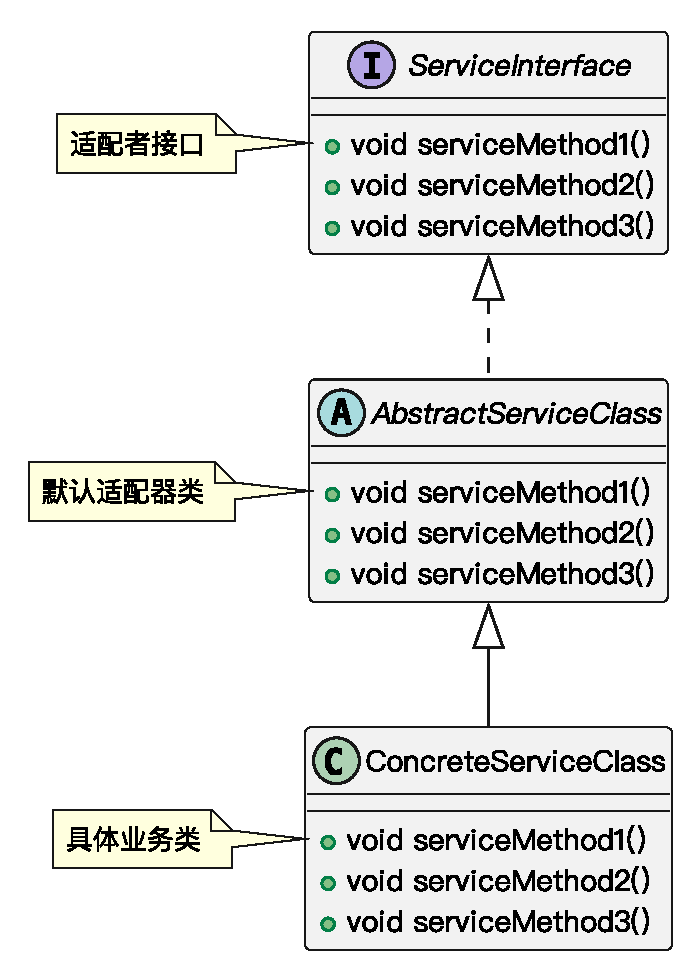
\includegraphics[width=0.97\linewidth]{images/适配器模式拓展1.eps}
	\end{minipage}
	}
    \hfill
    \subfloat{
    \begin{minipage}[c]{0.4\linewidth}
        \centering
        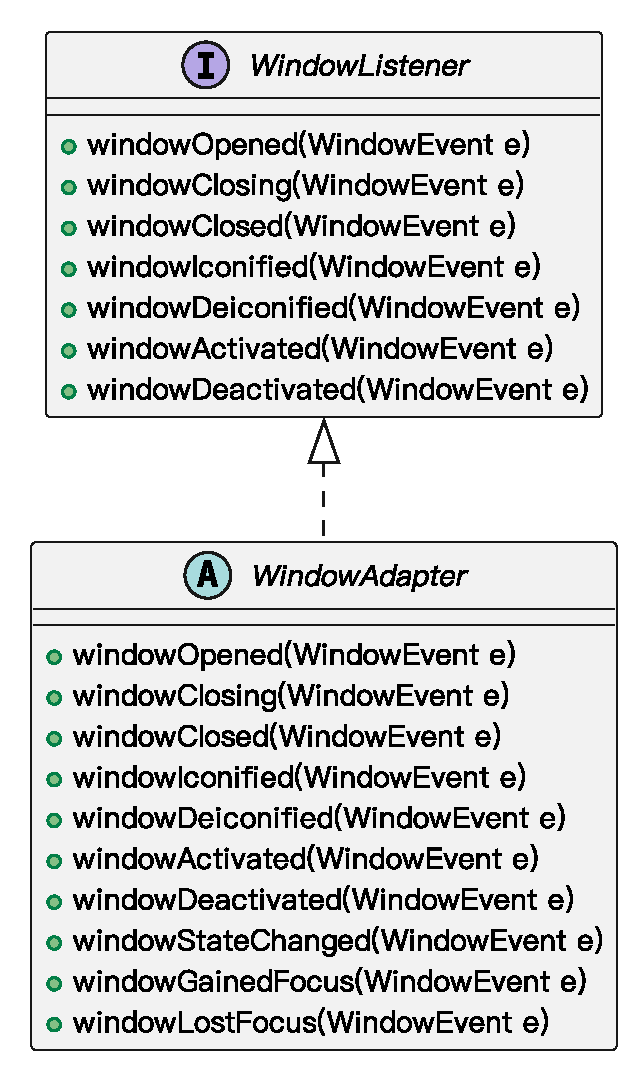
\includegraphics[width=0.97\linewidth]{images/适配器模式拓展2.eps}
    \end{minipage}
    }
	\centering
    \vspace{-1em}
\end{figure}

\paragraph*{双向适配器}~{} \par
在对象适配器的使用过程中,如果在适配器中同时包含对目标类和适配者类的引用,适配者可以通过它调用目标类中的方法,目标类也可以通过它调用适配者类中的方法,那么该适配器就是一个双向适配器。
\begin{figure}[H]
    \vspace{-0.5em}
	\centering
	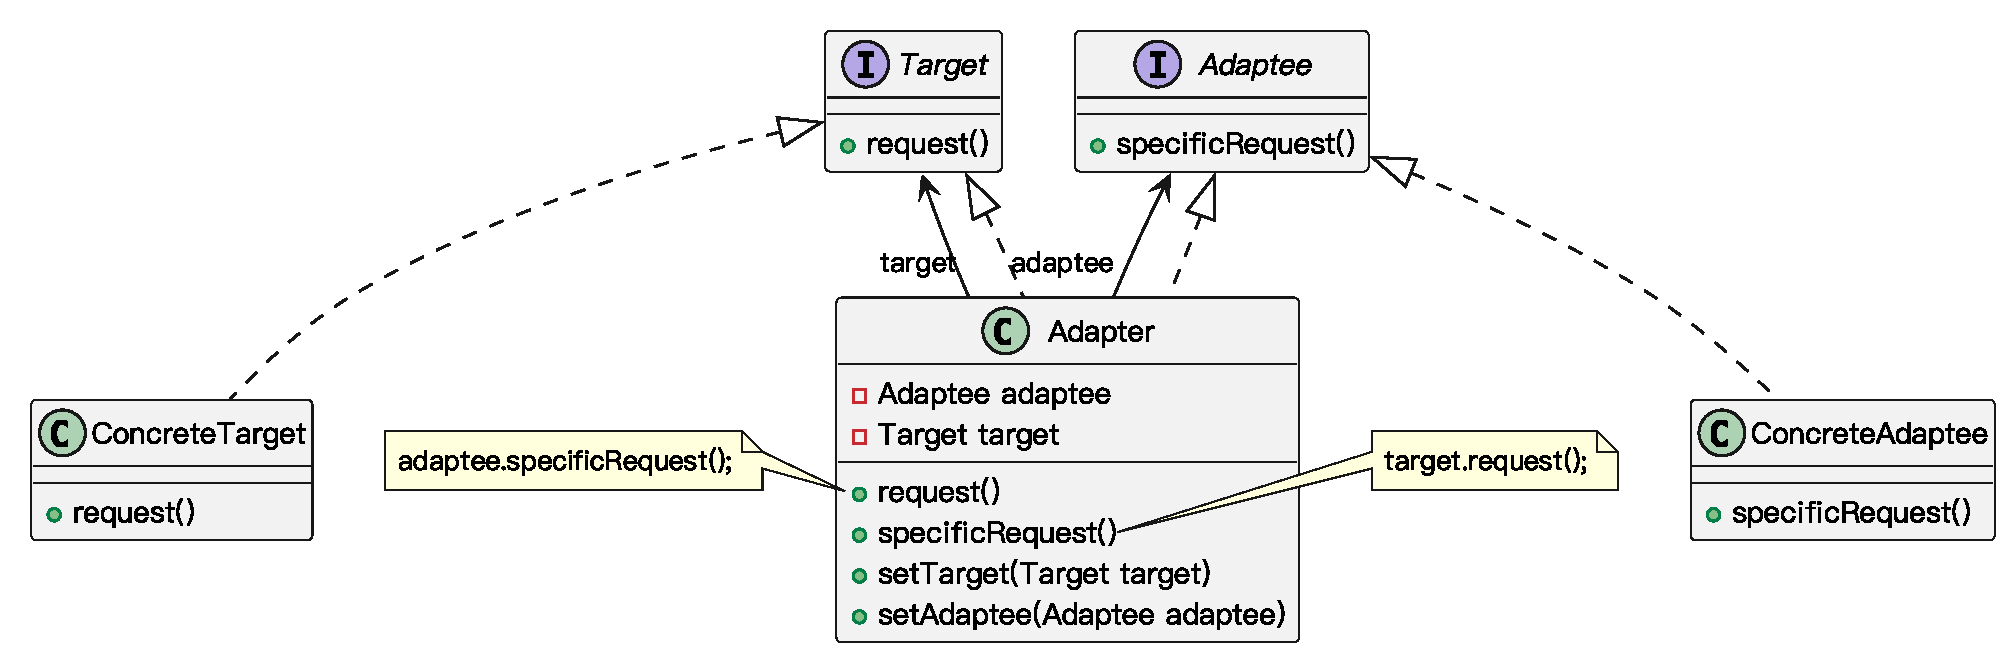
\includegraphics[width=\textwidth]{images/适配器模式拓展3.eps}
    \vspace{-1em}
\end{figure}


\subsection{组合模式}
对于\textbf{树形结构},当容器对象(如文件夹)的某一个方法被调用时,将遍历整个树形结构,寻找也包含这个方法的成员对象(可以是容器对象,也可以是叶子对象,如子文件夹和文件)并调用执行。\textbf{(递归调用)}

由于容器对象和叶子对象在功能上的区别,在使用这些对象的客户端代码中必须有区别地对待容器对象和叶子对象,而\textbf{实际上大多数情况下客户端希望一致地处理它们,因为对于这些对象的区别对待将会使得程序非常复杂}。

组合模式描述了如何将容器对象和叶子对象进行递归组合,使得用户在使用时无须对它们进行区分,可以一致地对待容器对象和叶子对象,这就是组合模式的模式动机。

\subsubsection{模式定义}
组合模式(Composite Pattern):组合多个对象形成树形结构以表示“整体-部分”的结构层次。组合模式对单个对象(即叶子对象)和组合对象(即容器对象)的使用具有一致性。

组合模式又可以称为整体-部分(Part-Whole)模式,属于对象的结构模式,它将对象组织到树结构中,可以用来描述整体与部分的关系。

\subsubsection{模式结构}
组合模式包含如下角色:
\vspace{-0.8em}
\begin{multicols}{2}
    \begin{itemize} 
        \item Component:抽象构件
        \item Leaf:叶子构件
        \item Composite:容器构件
        \item Client:客户类
    \end{itemize}
\end{multicols}
\vspace{-1em}

\begin{figure}[H]
    \vspace{-0.5em}
	\centering
	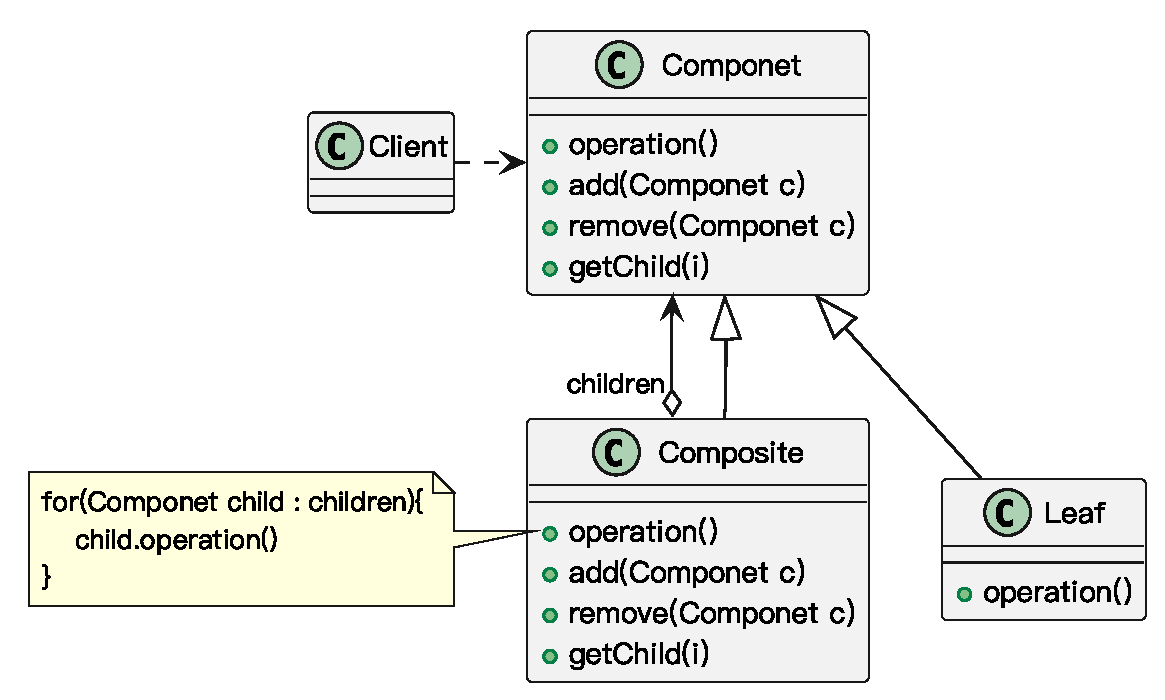
\includegraphics[width=0.6\textwidth]{images/组合模式结构.eps}
    \vspace{-1em}
\end{figure}

\subsubsection{模式分析}
组合模式的关键是\textbf{定义了一个抽象构件类},它既可以代表叶子,又可以代表容器,而\textbf{客户端针对该抽象构件类进行编程},无须知道它到底表示的是叶子还是容器,可以对其进行统一处理。

同时\textbf{容器对象与抽象构件类之间还建立一个聚合关联关系},在容器对象中既可以包含叶子,也可以包含容器,以此实现\textbf{递归}组合,形成一个\textbf{树形结构}。

文件系统组合模式结构图:
\begin{figure}[H]
	\centering
    \vspace{-0.5em}
	\subfloat{
	\begin{minipage}[c]{0.6\linewidth}
		\centering
		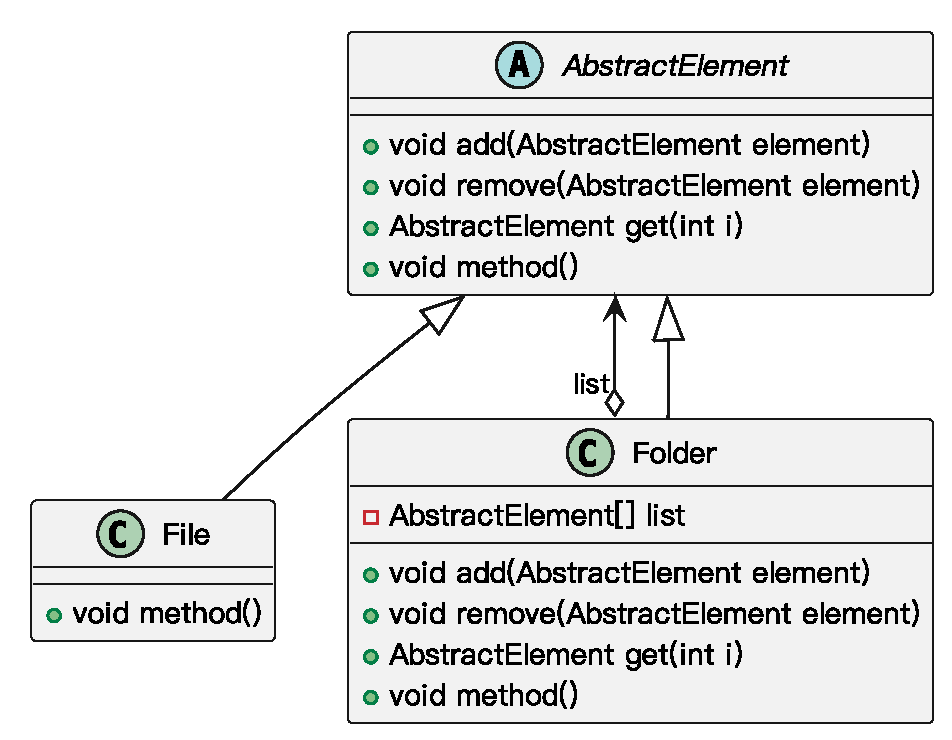
\includegraphics[width=0.95\linewidth]{images/组合模式分析.eps}
	\end{minipage}
	}
    \subfloat{
    \begin{minipage}[c]{0.35\linewidth}
        \centering
        \includegraphics[width=0.4\linewidth]{images/文件系统目录.png}
    \end{minipage}
    }
	\centering
    \vspace{-1em}
\end{figure}

组合模式典型代码:
\begin{figure}[H]
    \vspace{-0.5em}
	\centering
	\includegraphics[width=0.85\textwidth]{images/组合模式典型代码.pdf}
    \vspace{-1em}
\end{figure}

\subsubsection{模式实例}
水果盘:在水果盘(Plate)中有一些水果,如苹果(Apple)、香蕉(Banana)、梨子(Pear),当然大水果盘中还可以有小水果盘,现需要对盘中的水果进行遍历(吃),当然如果对一个水果盘执行“吃”方法,实际上就是吃其中的水果。使用组合模式模拟该场景。
\begin{figure}[H]
    \vspace{-0.5em}
	\centering
	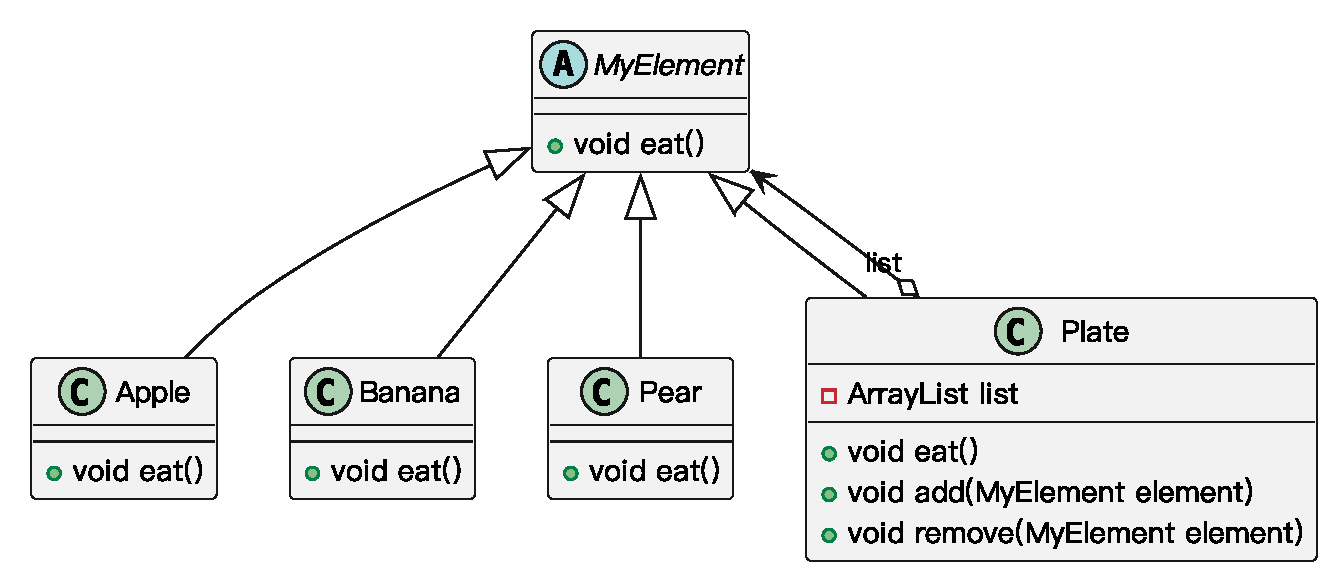
\includegraphics[width=0.72\textwidth]{images/组合模式实例1.eps}
    \vspace{-1em}
\end{figure}

文件浏览:文件有不同类型,不同类型的文件其浏览方式有所区别,如文本文件和图片文件的浏览方式就不相同。对文件夹的浏览实际上就是对其中所包含文件的浏览,而客户端可以一致地对文件和文件夹进行操作,无须关心它们的区别。使用组合模式来模拟文件的浏览操作。
\begin{figure}[H]
    \vspace{-0.5em}
	\centering
	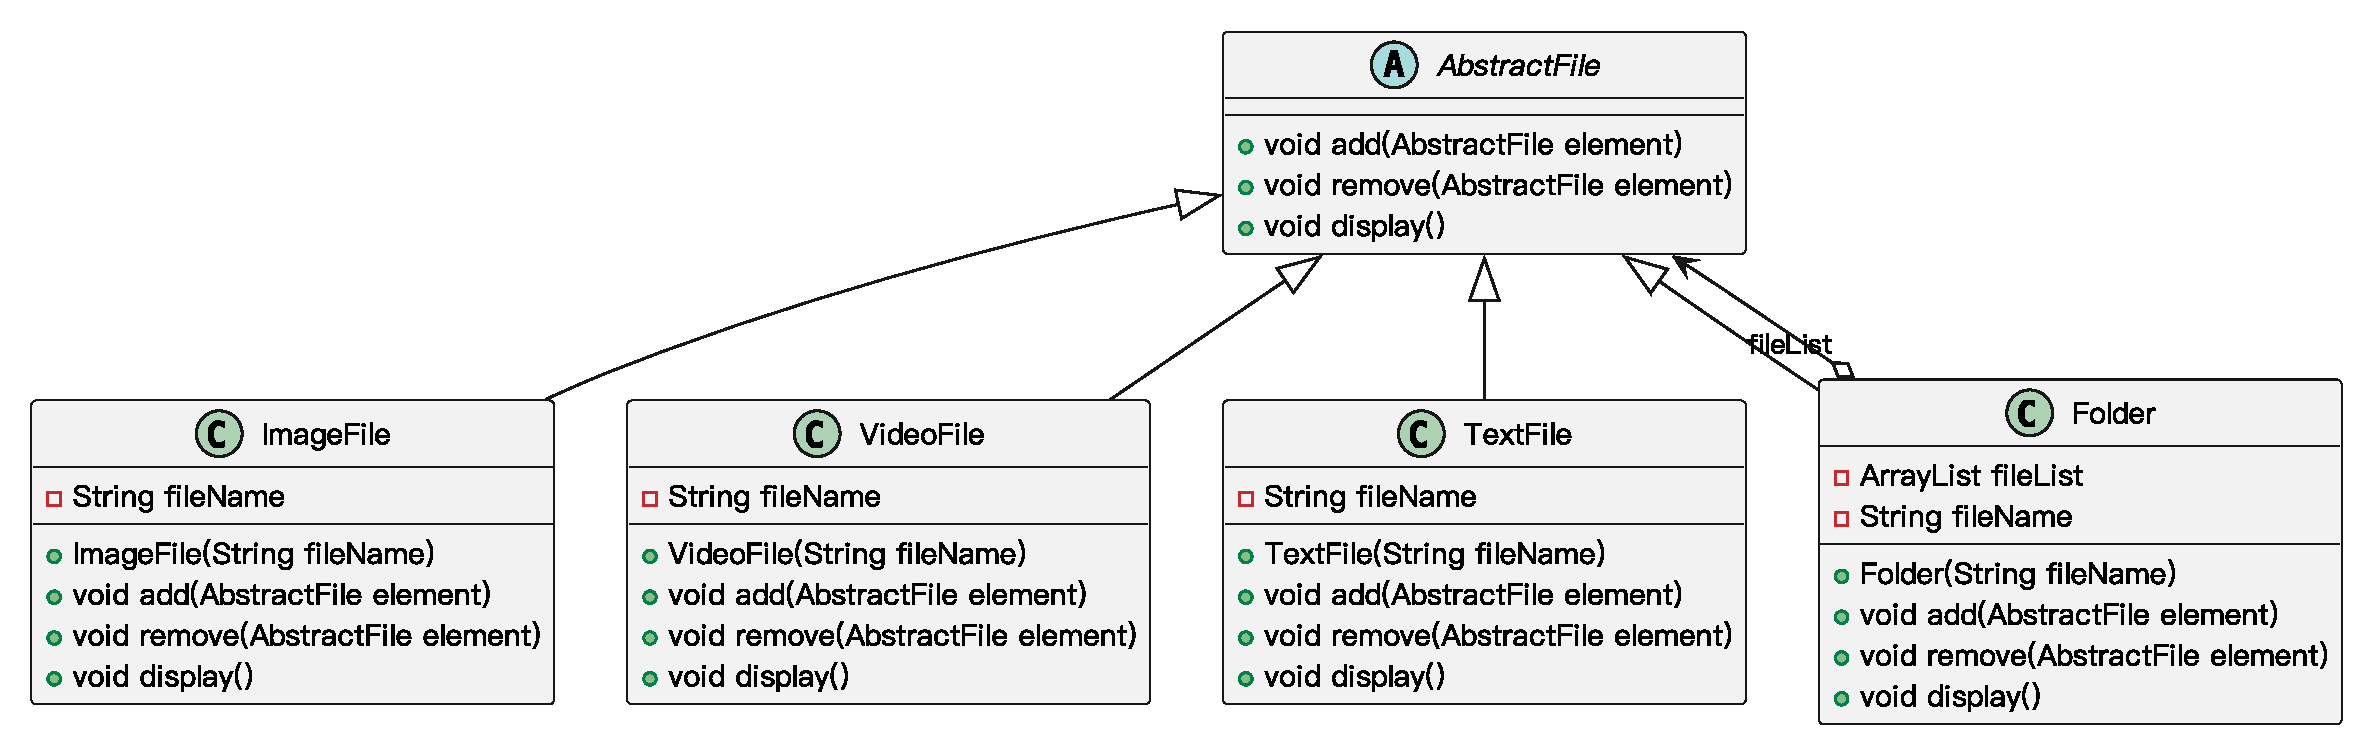
\includegraphics[width=\textwidth]{images/组合模式实例2.eps}
    \vspace{-1em}
\end{figure}

\subsubsection{模式优缺点}
组合模式的优点:
\begin{itemize}
    \item 可以清楚地定义\textbf{分层次的复杂对象},表示对象的全部或部分层次,使得增加新构件也更容易。
    \item 客户端调用简单,\textbf{客户端可以一致的使用组合结构或其中单个对象}。
    \item 定义了包含叶子对象和容器对象的\textbf{类层次结构},叶子对象可以被组合成更复杂的容器对象,而这个容器对象又可以被组合,这样不断递归下去,\textbf{可以形成复杂的树形结构}。
    \item \textbf{更容易在组合体内加入对象构件},客户端不必因为加入了新的对象构件而更改原有代码。组合模式
\end{itemize}

组合模式的缺点:
\begin{itemize}
    \item \textbf{使设计变得更加抽象},对象的业务规则如果很复杂,则实现组合模式具有很大挑战性,而且不是所有的方法都与叶子对象子类都有关联。
    \item 增加新构件时可能会产生一些问题,\textbf{很难对容器中的构件类型进行限制}。
\end{itemize}

\subsubsection{模式适用环境}
在以下情况下可以使用组合模式:
\begin{itemize}
    \item 需要表示一个\textbf{对象整体或部分层次},在具有整体和部分的层次结构中,希望通过一种方式忽略整体与部分的差异,可以一致地对待它们。
    \item 让客户能够忽略不同对象层次的变化,客户端可以\textbf{针对抽象构件编程},无须关心对象层次结构的细节。
    \item 对象的结构是动态的并且复杂程度不一样,但客户需要\textbf{一致地处理它们}。
\end{itemize}

\subsubsection{模式应用}
\ding{172} XML文档解析
\begin{figure}[H]
	\centering
    \vspace{-0.5em}
	\subfloat{
	\begin{minipage}[c]{0.58\linewidth}
		\centering
		\includegraphics[width=0.97\linewidth]{images/组合模式应用1.pdf}
	\end{minipage}
	}
    \subfloat{
    \begin{minipage}[c]{0.38\linewidth}
        \centering
        \includegraphics[width=0.97\linewidth]{images/组合模式应用2.pdf}
    \end{minipage}
    }
	\centering
    \vspace{-1em}
\end{figure}

\ding{173} 操作系统中的目录结构是一个树形结构,因此在对文件和文件夹进行操作时可以应用组合模式,例如杀毒软件在查毒或杀毒时,既可以针对一个具体文件,也可以针对一个目录。如果是对目录查毒或杀毒,将递归处理目录中的每一个子目录和文件。

\ding{174} JDK的AWT/Swing是组合模式在Java类库中的一个典型实际应用。
\begin{figure}[H]
    \vspace{-0.5em}
	\centering
	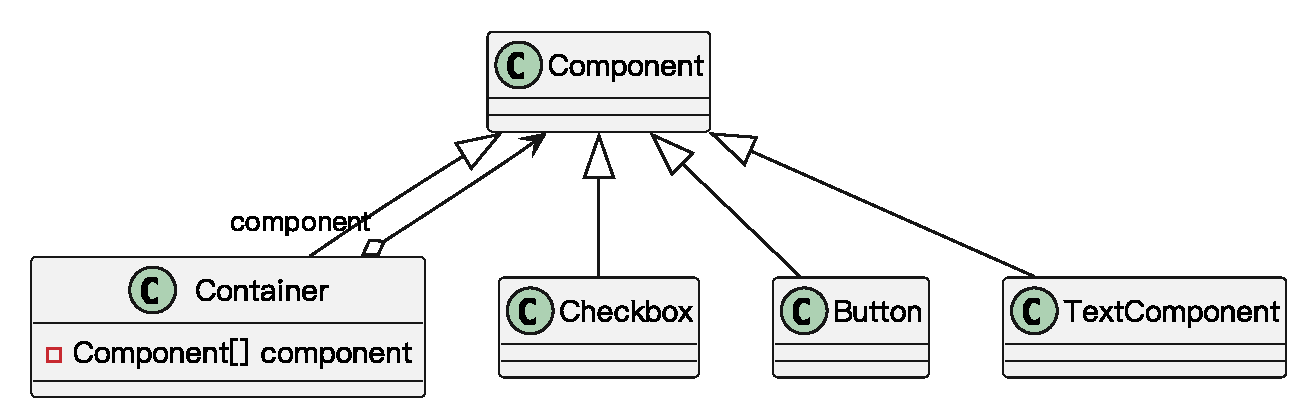
\includegraphics[width=0.65\textwidth]{images/组合模式应用3.eps}
    \vspace{-1em}
\end{figure}

\subsubsection{模式扩展}
更复杂的组合模式
\begin{figure}[H]
    \vspace{-0.5em}
	\centering
	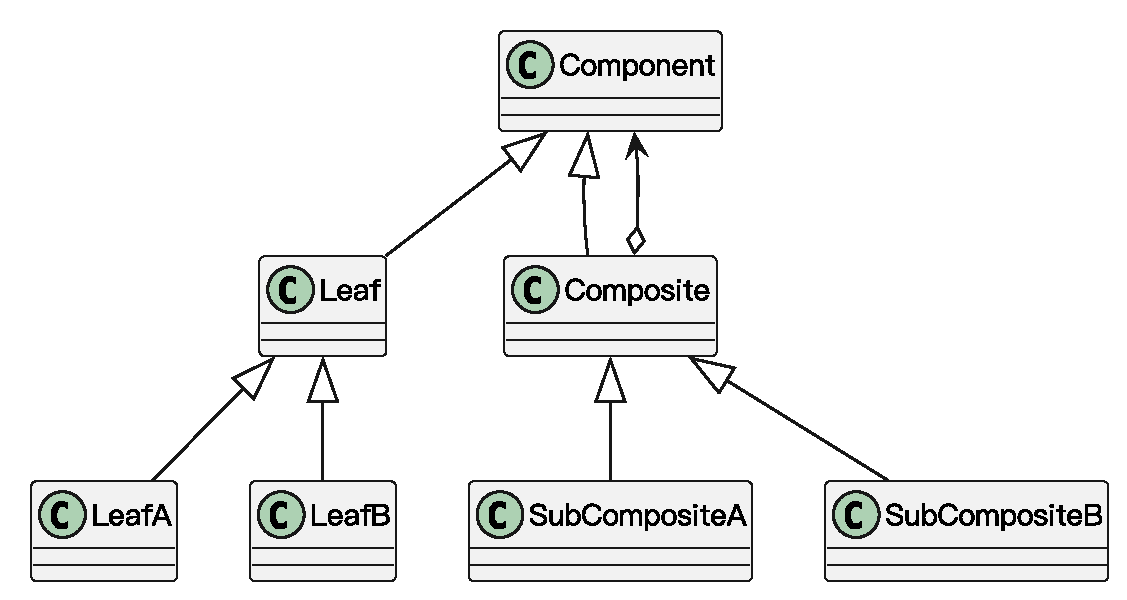
\includegraphics[width=0.57\textwidth]{images/更复杂的组合模式.eps}
    \vspace{-1em}
\end{figure}

透明组合模式
\begin{figure}[H]
    \vspace{-0.5em}
	\centering
	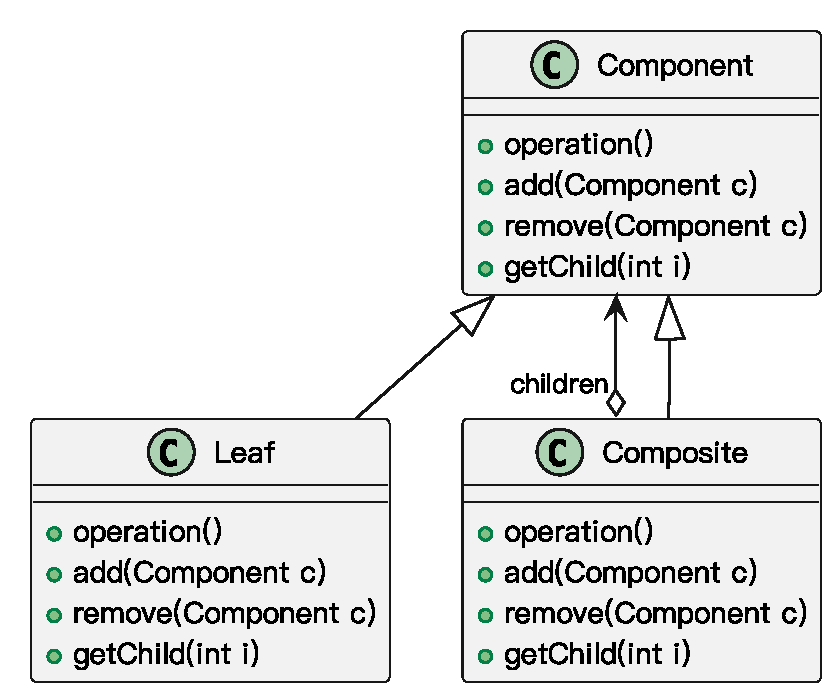
\includegraphics[width=0.45\textwidth]{images/透明组合模式.eps}
    \vspace{-1em}
\end{figure}

安全组合模式
\begin{figure}[H]
    \vspace{-0.5em}
	\centering
	\includegraphics[width=0.43\textwidth]{images/安全组合模式.eps}
    \vspace{-1em}
\end{figure}

